% poster cientifico slumx botnet analysis
\documentclass[25pt, a0paper, portrait]{tikzposter}

% paquetes necesarios
\usepackage[utf8]{inputenc}
\usepackage[english]{babel}
\usepackage{amsmath}
\usepackage{amsfonts}
\usepackage{amssymb}
\usepackage{graphicx}
\usepackage{booktabs}
\usepackage{array}
\usepackage{multirow}
\usepackage{pgfplots}
\pgfplotsset{compat=1.17}
\usetikzlibrary{arrows.meta, positioning, shapes.geometric, fit, calc}

% definir colores personalizados cybersecurity theme
\definecolor{NavyBlue}{HTML}{002347}
\definecolor{CyanTech}{HTML}{00A8E8}
\definecolor{AlertRed}{HTML}{C41E3A}
\definecolor{LightBg}{HTML}{F5F5F5}

% aplicar colores personalizados
\definecolorstyle{CyberSecurityStyle}{
    \definecolor{colorOne}{named}{NavyBlue}
    \definecolor{colorTwo}{named}{CyanTech}
    \definecolor{colorThree}{named}{AlertRed}
}{
    % background
    \colorlet{backgroundcolor}{LightBg}
    \colorlet{framecolor}{NavyBlue}
    % title colors
    \colorlet{titlefgcolor}{white}
    \colorlet{titlebgcolor}{NavyBlue}
    % block colors
    \colorlet{blocktitlebgcolor}{CyanTech}
    \colorlet{blocktitlefgcolor}{white}
    \colorlet{blockbodybgcolor}{white}
    \colorlet{blockbodyfgcolor}{black}
    % innerblock colors
    \colorlet{innerblocktitlebgcolor}{NavyBlue!20}
    \colorlet{innerblocktitlefgcolor}{black}
    \colorlet{innerblockbodybgcolor}{white}
    \colorlet{innerblockbodyfgcolor}{black}
    % note colors
    \colorlet{notefgcolor}{black}
    \colorlet{notebgcolor}{CyanTech!20}
    \colorlet{noteframecolor}{CyanTech}
}

% aplicar tema
\usecolorstyle{CyberSecurityStyle}
\usebackgroundstyle{Default}
\usetitlestyle{Default}
\useblockstyle{Default}

% titulo y autores
\title{\parbox{0.9\linewidth}{\centering Analysis of IoT Botnet Structure and Behavior:\\A Study Based on the Hitori (SlumX) Variant}}
\author{Ariel Matias Melo Pazmiño}
\institute{Universidad Internacional del Ecuador - Facultad de Ciencias Técnicas}

% logo placeholders
\titlegraphic{
    
\includegraphics[width=8cm]{university_logo.png}
    \hspace{10cm}
    
\includegraphics[width=8cm]{faculty_logo.png}
}

\begin{document}

\maketitle

% layout de 3 columnas
\begin{columns}

% ========== COLUMNA 1 ==========
\column{0.33}

\block{Abstract}{
The Internet of Things has fundamentally transformed cybersecurity, introducing billions of connected devices with minimal security measures. This research presents a comprehensive technical analysis of the SlumX botnet (Hitori variant) through static code analysis of the open-source repository.

\vspace{0.5em}
\textbf{Key Focus:} Understanding the evolution from simple credential attacks to sophisticated multi-architecture IoT malware with advanced evasion capabilities.
}

\block{Research Objectives}{
\textbf{General Objective:}
\begin{itemize}
    \item Conduct in-depth technical analysis of Hitori (SlumX) variant to understand modern IoT botnet threats
\end{itemize}

\vspace{0.5em}
\textbf{Specific Objectives:}
\begin{itemize}
    \item Analyze core architecture and operational framework
    \item Examine Command \& Control infrastructure design
    \item Identify and categorize DDoS attack vectors
    \item Evaluate multi-architecture support mechanisms
    \item Document evasion and anti-analysis techniques
    \item Assess IoT device scanning and exploitation capabilities
\end{itemize}
}

\block{Methodology}{
\textbf{Static Code Analysis Framework}

Analysis of the \texttt{mat1520/slumpx} repository using:

\begin{itemize}
    \item \textbf{Code Review:} Systematic examination of source files (\texttt{bot.c}, \texttt{server.c}, \texttt{scankill.c})
    \item \textbf{Control Flow Analysis:} Mapping execution paths and decision points
    \item \textbf{Threat Modeling:} Assessment of attack capabilities and defensive gaps
    \item \textbf{Architecture Analysis:} Cross-platform compilation and targeting strategies
\end{itemize}

\vspace{0.5em}
\textbf{Limitations:}
\begin{itemize}
    \item Static analysis cannot capture all runtime behaviors
    \item No testing on actual IoT devices
    \item Temporal snapshot of evolving malware
\end{itemize}
}

% ========== COLUMNA 2 ==========
\column{0.33}

\block{System Architecture}{
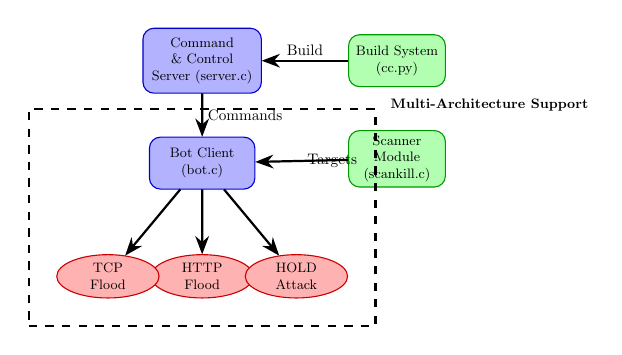
\begin{tikzpicture}[
    scale=0.55, transform shape,
    node distance=1.2cm and 1.5cm,
    >=Stealth,
    server/.style = {rectangle, draw=blue!80!black, fill=blue!30, text width=2.5cm, align=center, rounded corners, minimum height=1.5cm, font=\small},
    client/.style = {rectangle, draw=blue!80!black, fill=blue!30, text width=2.2cm, align=center, rounded corners, minimum height=1.2cm, font=\small},
    module/.style = {rectangle, draw=green!60!black, fill=green!30, text width=2cm, align=center, rounded corners, minimum height=1.2cm, font=\small},
    attack/.style = {ellipse, draw=red!80!black, fill=red!30, text width=1.6cm, align=center, minimum height=1cm, inner sep=1pt, font=\small},
    connection/.style = {draw, ->, thick, black}
]
    \node [server] (cnc) {Command \& Control Server (server.c)};
    \node [client, below=1cm of cnc] (bot) {Bot Client (bot.c)};
    \node [module, right=2cm of cnc] (build) {Build System (cc.py)};
    \node [module, below=1cm of build] (scanner) {Scanner Module (scankill.c)};
    \node [attack, below=1.5cm of bot] (http) {HTTP Flood};
    \node [attack, left=-0.2cm of http] (tcp) {TCP Flood};
    \node [attack, right=-0.2cm of http] (hold) {HOLD Attack};
    \node [draw, dashed, thick, black, inner sep=10pt, fit=(bot) (tcp) (hold) (http)] (container) {};
    \node [above right=-0.2cm and 0.2cm of container, font=\small\bfseries] {Multi-Architecture Support};
    \draw [connection] (cnc) -- node[right] {Commands} (bot);
    \draw [connection] (build) -- node[above] {Build} (cnc);
    \draw [connection] (scanner) -- node[right] {Targets} (bot);
    \draw [connection] (bot) -- (tcp);
    \draw [connection] (bot) -- (http);
    \draw [connection] (bot) -- (hold);
\end{tikzpicture}
}

\block{Infection Process Flow}{
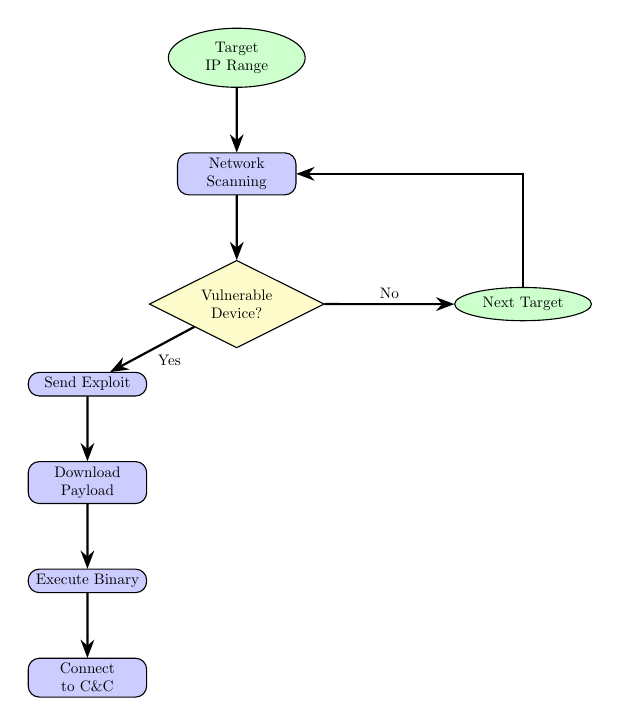
\begin{tikzpicture}[
    scale=0.55, transform shape,
    node distance=1.5cm, auto, >=Stealth,
    process/.style = {rectangle, draw, fill=blue!20, text width=2.5cm, text centered, rounded corners},
    decision/.style = {diamond, draw, fill=yellow!20, text width=2cm, text centered, aspect=2},
    data/.style = {ellipse, draw, fill=green!20, text width=2cm, text centered},
    arrow/.style = {draw, ->, thick}
]
    \node [data] (start) {Target IP Range};
    \node [process, below=of start] (scan) {Network Scanning};
    \node [decision, below=of scan] (vuln) {Vulnerable Device?};
    \node [process, below left=of vuln] (exploit) {Send Exploit};
    \node [process, below=of exploit] (payload) {Download Payload};
    \node [process, below=of payload] (execute) {Execute Binary};
    \node [process, below=of execute] (connect) {Connect to C\&C};
    \node [data, right=3cm of vuln] (next) {Next Target};
    
    \draw [arrow] (start) -- (scan);
    \draw [arrow] (scan) -- (vuln);
    \draw [arrow] (vuln) -- node {Yes} (exploit);
    \draw [arrow] (vuln) -- node {No} (next);
    \draw [arrow] (next) |- (scan);
    \draw [arrow] (exploit) -- (payload);
    \draw [arrow] (payload) -- (execute);
    \draw [arrow] (execute) -- (connect);
\end{tikzpicture}
}

\block{Multi-Architecture Support}{
\begin{center}
\begin{tabular}{ll}
\toprule
\textbf{Architecture} & \textbf{Target Devices} \\
\midrule
MIPS & Routers, Network Equipment \\
ARM & IoT Devices, Cameras \\
x86 & PC-based IoT Systems \\
PowerPC & Legacy Embedded Systems \\
SPARC & Enterprise IoT \\
M68k & Industrial Controllers \\
SH4 & Multimedia Devices \\
\bottomrule
\end{tabular}
\end{center}

\textbf{12 supported architectures} expanding attack surface across diverse IoT ecosystem.
}

% ========== COLUMNA 3 ==========
\column{0.33}

\block{Attack Vector Complexity}{
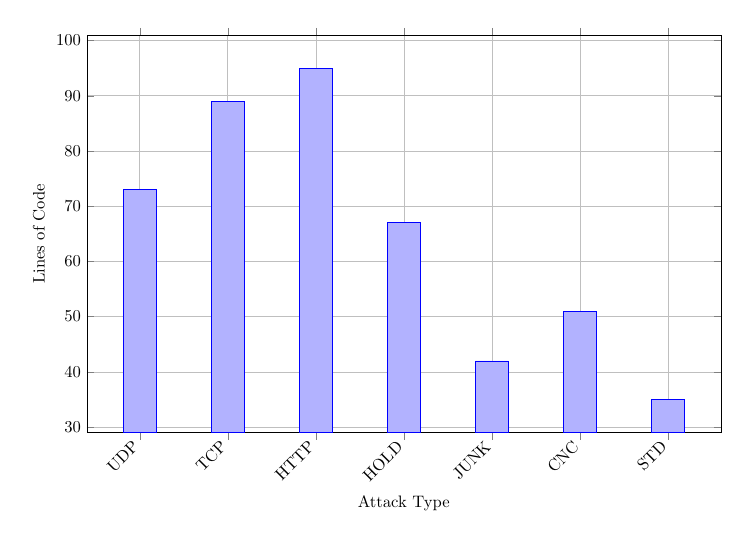
\begin{tikzpicture}[scale=0.6, transform shape]
\begin{axis}[
    xlabel={Attack Type},
    ylabel={Lines of Code},
    symbolic x coords={UDP,TCP,HTTP,HOLD,JUNK,CNC,STD},
    xtick=data,
    ybar,
    bar width=20pt,
    grid=major,
    width=15cm,
    height=10cm,
    x tick label style={rotate=45,anchor=east}
]
\addplot coordinates {(UDP,73) (TCP,89) (HTTP,95) (HOLD,67) (JUNK,42) (CNC,51) (STD,35)};
\end{axis}
\end{tikzpicture}

HTTP-based attacks show highest complexity (95 LOC) due to request crafting and user-agent randomization requirements.
}

\block{Vulnerability Assessment}{
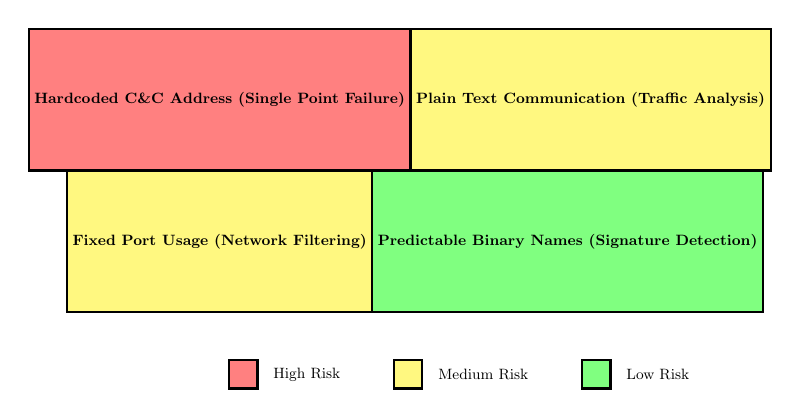
\begin{tikzpicture}[
    scale=0.6, transform shape,
    box/.style={rectangle, draw=black, thick, minimum width=5cm, minimum height=3cm, align=center, font=\small\bfseries, outer sep=0pt}
]
    \node[box, fill=red!50] (topleft) at (0,0) {Hardcoded C\&C Address (Single Point Failure)};
    \node[box, fill=yellow!50, right=0cm of topleft] (topright) {Plain Text Communication (Traffic Analysis)};
    \node[box, fill=yellow!50, below=0cm of topleft] (bottomleft) {Fixed Port Usage (Network Filtering)};
    \node[box, fill=green!50, right=0cm of bottomleft] (bottomright) {Predictable Binary Names (Signature Detection)};
    
    % leyenda
    \node[rectangle, draw=black, thick, minimum size=0.6cm, fill=red!50, below=1cm of bottomleft, xshift=0.5cm] (l1) {};
    \node[right=0.2cm of l1, font=\small] (t1) {High Risk};
    \node[rectangle, draw=black, thick, minimum size=0.6cm, fill=yellow!50, right=1cm of t1] (l2) {};
    \node[right=0.2cm of l2, font=\small] (t2) {Medium Risk};
    \node[rectangle, draw=black, thick, minimum size=0.6cm, fill=green!50, right=1cm of t2] (l3) {};
    \node[right=0.2cm of l3, font=\small] (t3) {Low Risk};
\end{tikzpicture}
}

\block{Key Findings}{
\begin{itemize}
    \item \textbf{Multi-architecture support:} 12 architectures (MIPS, ARM, x86, embedded systems) dramatically expanding attack surface
    \item \textbf{Advanced evasion:} Process masquerading, anti-analysis features, IoT-specific hiding techniques
    \item \textbf{Targeted exploitation:} Vendor-specific exploits and protocol-based attacks showing evolution from opportunistic to targeted attacks
    \item \textbf{Implementation flaws:} Buffer overflow vulnerabilities, hardcoded credentials, predictable attack patterns
\end{itemize}
}

\block{Conclusions}{
This analysis reveals significant advancement in IoT malware sophistication, particularly in multi-architecture targeting and evasion capabilities. The findings demonstrate evolution from opportunistic to targeted IoT attacks.

\vspace{0.5em}
\textbf{Future Work:}
\begin{itemize}
    \item Dynamic analysis frameworks for multi-architecture IoT malware
    \item Specialized detection technologies for resource-constrained devices
    \item Comparative analysis of botnet evolution patterns
\end{itemize}

\vspace{1em}
\begin{center}
\textbf{Research Paper QR Code}\\
\vspace{0.5em}
\framebox[5cm][c]{\rule{0pt}{5cm}\textbf{[QR CODE]}}
\end{center}
}

\end{columns}

\end{document}